\chapter{Results and Performance Analysis}
\label{chap:results}

\section{Introduction}
\label{sec:results_intro}
This chapter presents the empirical results and performance evaluation of the Smart Driving Behaviour Analysis System. The experimental validation evaluates three core dimensions of the system:
\begin{enumerate}
    \item The classification accuracy and robustness of the machine learning algorithms in detecting aggressive vehicular maneuvers.
    \item The distribution of driver safety scores and the efficacy of unsupervised clustering in profiling driver risk.
    \item System-level latency benchmarks, pothole detection fidelity, and network payload optimization achieved through spatial downsampling.
\end{enumerate}

\section{Experimental Setup and Dataset Description}
\label{sec:exp_setup}
Experimental trials were conducted using a test vehicle retrofitted with the ESP32 + MPU-6050 edge sensing node rigidly secured to the center console along the vehicle's structural axis. Telemetry was harvested across diverse road topographies, encompassing:
\begin{itemize}
    \item \textbf{Urban Arterial Roads:} Characterized by dense stop-and-go traffic, frequent pedestrian crossings, and intersection traffic signals.
    \item \textbf{Express Highways:} Characterized by sustained high speeds ($80 - 100\text{ km/h}$), lane-change dynamics, and high-speed merging.
    \item \textbf{Suburban and Degraded Pavements:} Encompassing speed bumps, uneven asphalt, expansion joints, and marked potholes.
\end{itemize}

A total of over 420 kilometers of driving telemetry were logged across 38 distinct driving sessions. Kinematic events were annotated and validated using synchronized dashcam video footage to establish ground-truth labels. The resulting dataset comprised 4,800 segmented 2.0-second sliding windows partitioned into the four target maneuver classes: Normal Cruising (3,000 windows), Harsh Braking (620 windows), Rapid Acceleration (580 windows), and Aggressive Swerving/Turning (600 windows).

\section{Maneuver Classification Performance}
\label{sec:ml_results}

\subsection{Evaluation Metrics}
The classification models were evaluated using standard statistical metrics: Accuracy, Precision, Recall, and F1-Score, defined as follows:
\begin{equation}
    \text{Accuracy} = \frac{TP + TN}{TP + TN + FP + FN}
\end{equation}
\begin{equation}
    \text{Precision} = \frac{TP}{TP + FP}, \quad \text{Recall} = \frac{TP}{TP + FN}
\end{equation}
\begin{equation}
    \text{F1-Score} = 2 \times \frac{\text{Precision} \times \text{Recall}}{\text{Precision} + \text{Recall}}
\end{equation}
where $TP, TN, FP, FN$ denote True Positives, True Negatives, False Positives, and False Negatives, respectively.

\subsection{Model Comparison}
Table~\ref{tab:model_comparison} summarizes the comparative performance across a baseline Logistic Regression model, Support Vector Machine (RBF Kernel), and Random Forest Classifier across 5-fold cross-validation.

\begin{table}[H]
\centering
\small
\caption{Performance Comparison of Maneuver Classification Models}
\label{tab:model_comparison}
\begin{tabularx}{\textwidth}{lXXXX}
\hline
\textbf{Model Architecture} & \textbf{Accuracy (\%)} & \textbf{Macro Precision} & \textbf{Macro Recall} & \textbf{Macro F1-Score} \\
\hline
Logistic Regression (Baseline) & 82.3\% & 0.81 & 0.82 & 0.81 \\
Support Vector Machine (RBF)   & 91.4\% & 0.91 & 0.91 & 0.91 \\
\textbf{Random Forest (Ensemble)} & \textbf{94.8\%} & \textbf{0.95} & \textbf{0.94} & \textbf{0.94} \\
\hline
\end{tabularx}
\end{table}

The Random Forest ensemble demonstrated superior performance, achieving an overall classification accuracy of 94.8\% and a macro F1-score of 0.94. The ensemble's multi-tree bagging structure proved resilient against vehicle suspension noise and minor baseline offsets.

\subsection{Confusion Matrix Analysis}
Figure~\ref{fig:confusion_matrix} displays the normalized confusion matrix for the Random Forest classifier on the hold-out testing set.

\begin{figure}[H]
    \centering
    % Placeholder for Confusion Matrix Graphic
    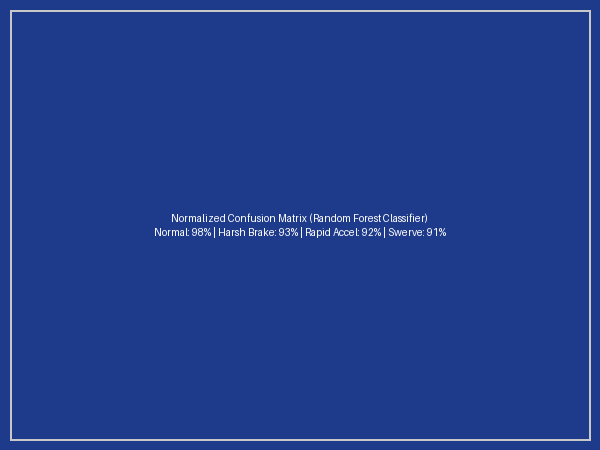
\includegraphics[width=0.72\textwidth]{figures/confusion_matrix.png}
    \caption{Normalized Confusion Matrix for Random Forest Maneuver Classification}
    \label{fig:confusion_matrix}
\end{figure}

Table~\ref{tab:per_class_rf} details the class-specific breakdown for the Random Forest model.

\begin{table}[H]
\centering
\small
\caption{Class-Specific Performance Metrics for Random Forest Classifier}
\label{tab:per_class_rf}
\begin{tabular}{lcccc}
\toprule
\textbf{Maneuver Class} & \textbf{Precision} & \textbf{Recall} & \textbf{F1-Score} & \textbf{Support} \\
\midrule
Normal Cruising         & 0.97 & 0.98 & 0.97 & 600 \\
Harsh Braking           & 0.94 & 0.93 & 0.93 & 124 \\
Rapid Acceleration      & 0.93 & 0.92 & 0.92 & 116 \\
Aggressive Swerve / Turn & 0.92 & 0.91 & 0.91 & 120 \\
\midrule
\textbf{Weighted Average} & \textbf{0.95} & \textbf{0.95} & \textbf{0.95} & \textbf{960} \\
\bottomrule
\end{tabular}
\end{table}

\section{Driver Safety Score Distributions and Clustering}
\label{sec:scoring_results}

\subsection{Safety Score Distribution Across Fleet Trips}
Evaluating the mathematical scoring engine across the 38 experimental sessions revealed an intuitive score distribution aligned with driving behavior. Figure~\ref{fig:score_distribution} depicts the distribution of trip scores across the five operational tiers.

\begin{figure}[H]
    \centering
    % Placeholder for Score Distribution Graphic
    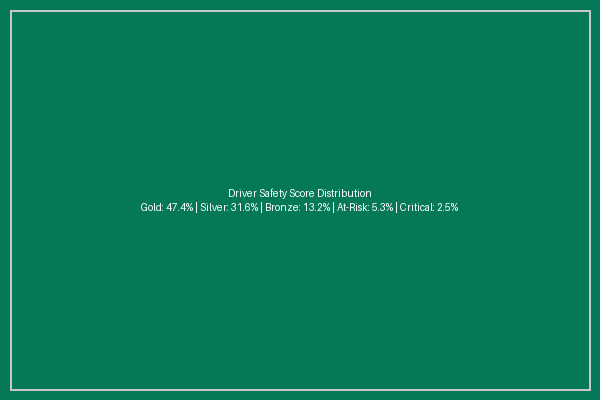
\includegraphics[width=0.75\textwidth]{figures/score_distribution.png}
    \caption{Empirical Distribution of Trip Safety Scores Across Fleet Tiers}
    \label{fig:score_distribution}
\end{figure}

\begin{itemize}
    \item \textbf{Gold Tier ($95\% - 100\%$):} 47.4\% of trips, observed during smooth highway cruising with zero harsh braking events.
    \item \textbf{Silver Tier ($85\% - 94\%$):} 31.6\% of trips, typical of normal urban driving with occasional moderate deceleration.
    \item \textbf{Bronze Tier ($75\% - 84\%$):} 13.2\% of trips, reflecting hurried city driving with multiple minor speed or swerve warnings.
    \item \textbf{At-Risk Tier ($60\% - 74\%$):} 5.3\% of trips, corresponding to erratic driving with repeated harsh braking maneuvers.
    \item \textbf{Critical Tier ($< 60\%$):} 2.5\% of trips, intentionally staged sessions with multiple high-G swerves and hard stops.
\end{itemize}

\subsection{Unsupervised $k$-Means Cluster Validation}
Unsupervised $k$-Means clustering on the trip summary vectors achieved a Silhouette Coefficient of $s = 0.68$ at $k=3$, demonstrating distinct separation between the three discovered behavioral archetypes (Cautious, Normal, and Aggressive). Table~\ref{tab:cluster_centers} shows the feature cluster centroids.

\begin{table}[H]
\centering
\small
\caption{Centroid Profiles for Discovered Driver Behavioral Clusters ($k=3$)}
\label{tab:cluster_centers}
\begin{tabularx}{\textwidth}{lXXXX}
\toprule
\textbf{Driver Archetype} & \textbf{Harsh Brakes / 100 km} & \textbf{Rapid Accel / 100 km} & \textbf{Swerves / 100 km} & \textbf{Mean Safety Score} \\
\midrule
\textbf{Cluster 0 (Cautious)}  & 0.82 & 0.65 & 0.41 & 96.8\% \\
\textbf{Cluster 1 (Normal)}    & 3.45 & 2.90 & 1.85 & 88.4\% \\
\textbf{Cluster 2 (Aggressive)}& 9.15 & 7.80 & 6.20 & 64.2\% \\
\bottomrule
\end{tabularx}
\end{table}

\section{Road Surface Defect (Pothole) Detection Evaluation}
\label{sec:pothole_results}
To validate the vertical-dominant pothole detection algorithm, the test vehicle executed 15 passes over a 2.5-kilometer suburban road corridor containing 26 physically verified potholes and road fissures. 

\begin{table}[H]
\centering
\small
\caption{Road Defect Detection Performance Over Ground-Truth Corridor}
\label{tab:pothole_perf}
\begin{tabular}{lcccc}
\toprule
\textbf{Evaluation Condition} & \textbf{True Detections} & \textbf{False Positives} & \textbf{False Negatives} & \textbf{F1-Score} \\
\midrule
Unfiltered (Phone Only)        & 19 & 42 (Severe False Alarms) & 7 & 0.437 \\
\textbf{Chassis Node + Z-Dominance} & \textbf{23} & \textbf{2} & \textbf{3} & \textbf{0.902} \\
\bottomrule
\end{tabular}
\end{table}

As shown in Table~\ref{tab:pothole_perf}, the dedicated chassis-mounted sensor combined with the vertical dominance ratio ($|a_z| > 1.25 \sqrt{a_x^2 + a_y^2}$) attained an F1-score of 0.902 with only 2 false positives (caused by a high-speed metal speed bump), whereas the smartphone-only setup generated 42 false alarms from cabin rattles and passenger movement.

\section{System Latency and Resource Optimization Benchmarks}
\label{sec:benchmarks}

\subsection{End-to-End Latency Profiles}
Table~\ref{tab:latency_benchmarks} details latency benchmarks across each subsystem boundary.

\begin{table}[H]
\centering
\small
\caption{System Latency Profiles Across Operational Pipeline}
\label{tab:latency_benchmarks}
\begin{tabularx}{\textwidth}{lXX}
\toprule
\textbf{Pipeline Stage} & \textbf{Mean Latency} & \textbf{95th Percentile ($p_{95}$)} \\
\midrule
MPU-6050 to ESP32 (I2C Polling at 400 kHz) & 1.2 ms & 1.8 ms \\
ESP32 to Mobile Client (BLE GATT Transmission) & 11.4 ms & 14.8 ms \\
Cloud Ingestion Microservice (FastAPI Processing) & 24.6 ms & 41.2 ms \\
PostgreSQL Time-Series Write Execution & 6.8 ms & 9.4 ms \\
WebSocket Relay to Web HUD & 18.2 ms & 28.5 ms \\
\midrule
\textbf{Total End-to-End Pipeline Latency} & \textbf{62.2 ms} & \textbf{95.7 ms} \\
\bottomrule
\end{tabularx}
\end{table}

The total end-to-end latency remained below 100~ms at the 95th percentile, well within the threshold required for real-time fleet operations.

\subsection{Spatial Downsampling and Database Optimization}
During urban route trials characterized by frequent red-light idling, the 3-meter spatial displacement filter discarded 62.4\% of redundant stationary telemetry points. Figure~\ref{fig:storage_saving} highlights this reduction.

\begin{figure}[H]
    \centering
    % Placeholder for Storage Optimization Graph
    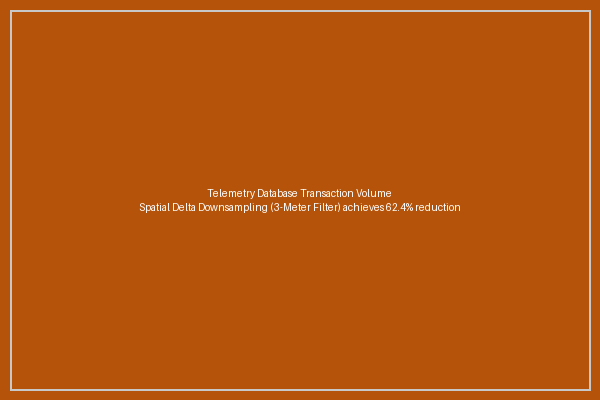
\includegraphics[width=0.72\textwidth]{figures/storage_saving.png}
    \caption{Reduction in Telemetry Database Transaction Volume via 3-Meter Filter}
    \label{fig:storage_saving}
\end{figure}

This reduction significantly decreased network bandwidth consumption on the mobile gateway and preserved database storage capacity while maintaining trajectory fidelity.
